\setchapterpreamble[ur][.6\textwidth]{%
\dictum[Heraclitus cited by Plato, \textit{Cratylus} (4-5th century BCE)]{%
All entities move and nothing remains still.}\vskip1em
\dictum[Frank Herbert, \textit{Dune} (1965)]{%
It is impossible to live in the past, difficult to live in the present and a waste to live in the future.}\vskip1em
}


\chapter[\texorpdfstring{Chapter 5 \\ Fluctuating selection but no fluctuating evolution in a wild rodent population}{Chapter 5 -- Fluctuating selection but no fluctuating evolution in a wild rodent population}]{Fluctuating selection but no fluctuating evolution in a wild rodent population}
\chaptermark{Fluctuating selection}
\label{chap:flusel}

\section{Abstract}
Temporal fluctuations in the strength and direction of selection are often suggested to slow down evolution, both over geological and contemporary time-scales. The prevalence of fluctuating selection and its relevance for evolutionary dynamics remains unclear however, especially on contemporary time scales: Unbiased empirical estimates of variation in selection are still scarce, and the question of how much variation in selection translates into variation in genetic change has been largely ignored.
Using long-term individual-based data for a wild rodent population, we quantify the amount of fluctuating selection on body mass. Subsequently, we estimate the evolutionary dynamics of mass, and test for a link between fluctuating selection and evolution. 
We show that, over the past 10 years, phenotypic selection on body mass has fluctuated significantly. While this variation is largely the result of variation in fertility rather than viability selection, viability selection is the main driver of adaptive evolution in this system. Accordingly, we found that the strength and direction of genetic change remained stable over the study period. Thus, the rate of genetic change was similar in years where total selection favoured heavier or lighter individuals.
These results demonstrate that, over shorter time-scales, fluctuating selection is not necessarily evolutionary relevant. 

\section*{Introduction}
Selection shapes biodiversity in time and space, explaining the general match between organisms and their environment \parencite{Darwin1859,Endler1986}. Linking the sources of natural and sexual selection to the dynamics of genetic evolution has been a focus of evolutionary biology during the last century \parencite[e.g.][]{Fisher1958}, but for most of the 20th century this goal has been hampered by the lack of an unified framework to quantify selection \parencite{Wade2006}. This changed with the development of regression-based methods to measure the strength and direction of selection \parencite{Lande1979,Lande1983}, which have enabled the estimation of selection gradients in a large variety of traits and biological systems \parencite{Kingsolver2001,Stinchcombe2008}. This bonanza of estimates has shown that directional selection is stronger and more common than balancing selection, for both morphological and life-history traits \parencite{Kingsolver2001,Hereford2004}. At first sight, this pattern is contrary to expectations \parencite{Kingsolver2011}: As most traits are heritable \parencite{Postma2014}, they are predicted to evolve towards their fitness optimum, with directional selection progressively being replaced by balancing selection. However, most traits evolve only very slowly and within a limited phenotypic range \parencite{Hendry1999, Merila2001, Brookfield2016}. 

One explanation for this paradox is that fitness landscapes are not constant over time, and populations are evolving towards a continuously changing fitness optimum \parencite{Fisher1947,Lande1976}. Whereas at any point in time directional selection may be strong, average selection gradients may be weaker, and if selection fluctuates not only in strength but also in direction, average selection may even be zero (Figure \ref{fig:concept} (A-C)). Given that fluctuating selection may slow down evolutionary adaptation, or even bring it to a halt \parencite{Jones2004,Estes2007}, it constitutes an appealing explanation for the commonly observed lack of evolutionary change, i.e. evolutionary stasis, as well as for the commonness of directional selection \parencite{Merila2001,Robinson2008,Bell2010a}. However, although fluctuating selection as an explanation for ``macro-evolutionary'' stasis is gaining theoretical and empirical support  \parencite{Uyeda2011, Estes2007, Voje2015}, our understanding of the importance of fluctuations in selection in shaping the evolutionary dynamics of natural populations on a much smaller time scale, e.g. from year one year to the next, is hampered by the lack of a clear answer to two questions: (i) Does phenotypic selection really fluctuate, in strength and/or direction, over short time scales? (ii) If it does, do these fluctuations translate into fluctuations, in speed and/or direction, of genetic change?

The first question seemingly received a positive answer with the publication of a synthetic analysis of temporal replicates of selection from 89 studies, which came to the conclusion that phenotypic selection does indeed vary and reverses its direction among years \parencite{Siepielski2009}. However, \cite{Morrissey2012flusel} showed that most of these fluctuations can be ascribed to sampling variation, and that when this is accounted for, directional selection is in fact remarkably constant over time, both in magnitude and direction. 

Instead of estimating the variance of the distribution of temporal estimates of selection, as in \parencite{Siepielski2009}, tests for fluctuating selection must estimate the variance of the temporal distribution of selection \cite{Morrissey2012flusel}. As of yet, \cite{Chevin2015b} are among the few to have done this: Using a random regression approach, they found that phenotypic selection on laying date fluctuated over a short time period in a population of great tits (\textit{Parus major} Linnaeus, 1758). The generality of this finding however needs to be confirmed across across a wider range of species, populations and traits, using the same robust approach. 

\begin{figure}
	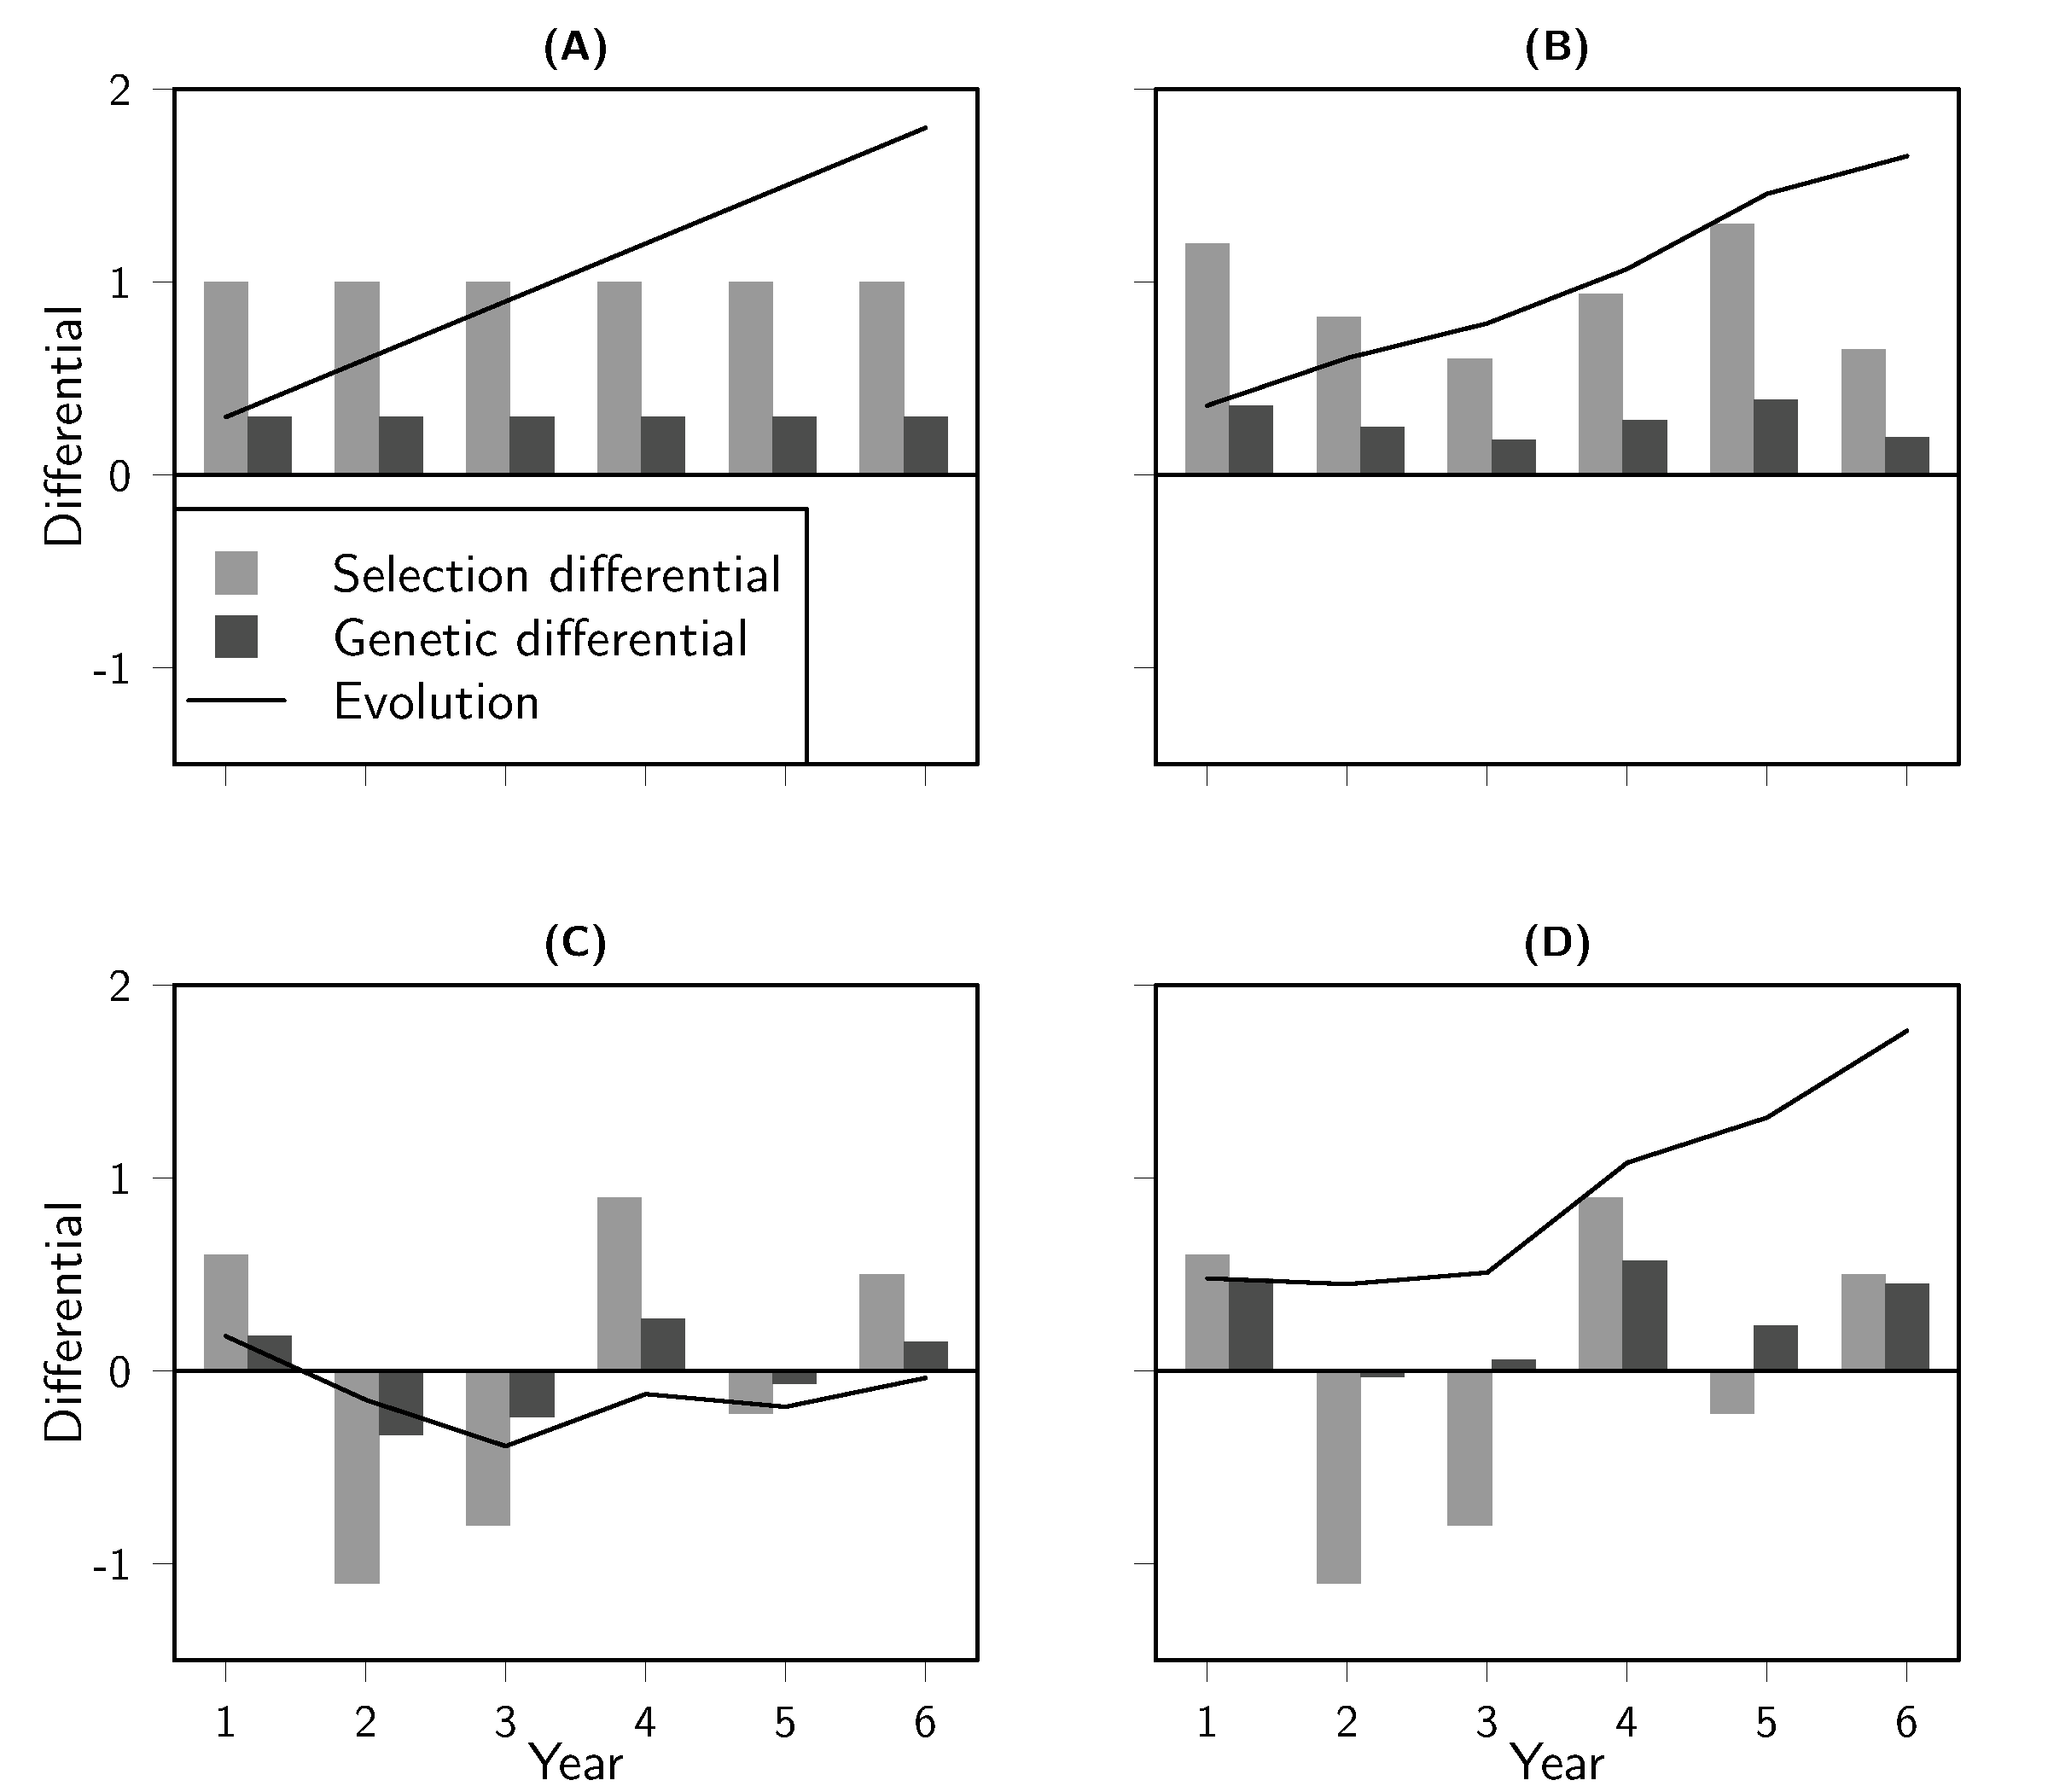
\includegraphics[width=\textwidth]{FiguresFluSel/concetpualplot-1}
	\caption{Evolutionary change under constant and fluctuating selection regimes. 
	In \textbf{(A)}, selection is constant among years. Following the breeder's equation, the genetic differential (i.e. the response to selection) is equal to the product of the selection differential and the heritability, which is here set to $0.3$. The resultant cumulative response to selection, i.e the evolutionary trajectory, is described by a straight line. 
	In \textbf{(B)}, selection fluctuates but does not reverse, and mean selection and the rate of evolution are only slightly reduced compared to \textbf{(A)}.
	In \textbf{(C)}, selection fluctuates and reverses, resulting in fluctuating and reversing evolution, and thereby evolutionary stasis over the time frame considered. 
	In \textbf{D}, selection fluctuates and reverts as in \textbf{C}, but selection is partly non-causal and mediated by an unobserved environmental factor (i.e. a key assumption of the breeder's equation is violated). As a consequence, selection and evolution are uncoupled and despite fluctuating selection the rate of evolution is similar to \textbf{(A)}.}
	\label{fig:concept}
\end{figure}

%%%

In addition to showing statistically significant variation in selection, two more points must be investigated to assess the evolutionary relevance of fluctuating selection. First, the precise pattern of fluctuation matters. Even in the presence of fluctuating selection, evolution will only come to a halt if the direction of selection changes regularly and the mean selection differential equals zero \parencite{Blanckenhorn2000, Hunt2004a, Morrissey2012flusel} (see Figure \ref{fig:concept} (B)). Second, phenotypic selection, defined as a non-null phenotypic covariance between a trait and relative fitness, does not necessarily lead to an evolutionary response \parencite{Rausher1992} (see Figure \ref{fig:concept} (D)): Estimates of phenotypic selection provide a poor predictor of genetic change when the assumptions of the breeder's equation are violated, and in particular when selection is disproportionally dominated by an environmental covariance between the trait of interest and fitness \parencite{Price1989,Rausher1992,Bonnet2016}.

While this is one of the general explanations for apparent evolutionary stasis, it is particularly relevant within the context of fluctuating selection: As fluctuating selection is often thought to be driven by environmental fluctuations \parencite{Bell2010a, Chevin2014}, these may disproportionally shape the environmental component of selection. If fluctuating selection is not the result of fluctuations in the causal effects of the focal trait on fitness, it will not result in fluctuations in the additive genetic covariance between the trait and fitness, i.e. in fluctuating evolution \parencite{Robertson1966, Price1970, Morrissey2012sts}. Hence, fluctuating selection affects evolutionary dynamics only if the variation in the sign and strength of selection is, at least partly, coupled to variation in the sign and pace of genetic change.

Here we take advantage of the ten-year long monitoring of a population of snow voles (\textit{Chionomys nivalis} Martins, 1842) to i) quantify fluctuating selection on body mass, ii) describe the temporal dynamics of evolution in mass, and iii) quantify the relationship between fluctuating selection and evolution. To this end, we first estimate directional selection on a year-to-year basis to quantify the variation in selection estimates. We then explicitly model these fluctuations of directional selection within a random regression framework in order to account for sampling variance. Based on the sign of annual selection estimates, as well as on the ratio of the variance in selection over the mean strength of selection, we also assess the probability of selection reversal. These analyses are performed for total selection, as well as for fertility and viability selection separately. 
Subsequently, we use a quantitative genetic framework to describe the general pattern of evolution over the study period, and estimate the rate of evolution of mass on a year-to-year basis. 
Finally, we combine analyses of selection and estimations of evolution to assess the coupling between variation in the strength and sign of selection and evolution.


%%%%%%%%%%%%%%%%%%%%%%%%%%%%%%%%%%%%%%%%%%%%%%%%%%%%%%%%%%%%%%%%%%%%%%%%%%%%%%%%%%%%%%%%%%%%%%%%%%%
%%%%%%%%%%%%%%%%%%%%%%%%%%%%%%%%%%%%%%%%%%%%%%%%%%%%%%%%%%%%%%%%%%%%%%%%%%%%%%%%%%%%%%%%%%%%%%%%%%%
\section*{Material and methods}
\subsection*{Study population}
Since 2006, a wild population of snow voles (\textit{Chionomys nivalis} Martins, 1842) has been monitored intensively. This population is located in the Swiss Alps, near Chur (N$46^\circ48'$, E$9^\circ34'$; 2,030 m.a.s.l.). The study area consists of 5 ha of scree with sparse vegetation, surrounded by meadows, forest and a steep cliff. Because the snow vole shows an overwhelming preference for rocky environments \parencite{Janeau1997, Luque-larena2002}, the monitored population is ecologically fairly isolated. 
Every year, snow voles have been live-trapped during two to five trapping sessions, between mid-June and early October. To this end, the study area is overlaid with a $10\times10$ m grid consisting of a total of 559 cells with stable geographic coordinates. A trapping session consists of four trapping nights, necessary to cover all four quarters of the study area.

During each trapping session, a Longworth trap (catch-and-release trap, Penlon Ltd, Oxford, UK) filled with hay and baited with apple, hamster food and peanut butter is placed in every cell. Individuals captured for the first time are ear-clipped (2mm diameter, thumb type punch, Harvard Apparatus, Massachusetts, USA) and individually marked with a subcutaneous PIT tag (ISO transponder, Tierchip Dasmann, Tecklenburg, Germany). Ear-clips are preserved in 95\% ethanol + 5\% TE. For each capture, we record individual identity, geographic coordinates, body mass, body length, tail length, sex and age.

Ear clips are stored at $-20^\circ$C until DNA extraction. All individuals are genotyped for 18 autosomal microsatellites, using snow vole-specific primers \parencite{Wandeler2008, Garcia-Navas2015}. In addition, the sex of all individuals is confirmed by sequencing the \textit{Sry} locus \parencite{Gubbay1990}. Finally, we sequence the mitochondrial control region, and all males are genotyped for one Y-linked microsatellite and three Y-linked insertion-deletions \parencite{Wandeler2011}.
Based on the autosomal microsatellite genotypes, we reconstruct the pedigree of the population using the maximum likelihood based program COLONY \parencite{Wang2004,Jones2010} and a Bayesian R package MasterBayes \parencite{Hadfield2006,R2016}. The consistency of the pedigree is then checked for consistency using the Y-linked markers and the mitochondrial haplotypes. This procedure allows the identification of most of the parental links (91\%) as well as the identification of likely immigrants (individuals first captured as adults and with two unknown parents).This high-quality pedigree is used to define annual reproductive success and lifetime reproductive success, as well as to estimate the relatedness among all pairs of individuals.

A mark-recapture analysis has shown that between-session recapture probabilities are very high (adults: 92.4\% $\pm1.1$; juveniles: 81.1\%$\pm3.0$). Therefore, the year-to-year recapture probability is effectively 1, which means that the non-capture of an individual in a given year can be directly equated with death or permanent immigration without the need for mark-recapture modeling \parencite{Garcia-Navas2015}.

\subsection*{Fitness measures}
We considered three measures of fitness: (i) survival from one year to the next, $\phi_{i,t}$, based on whether an individual $i$ observed in year $t$ is observed again in year $t+1$ ($\phi_{i,t}=1$) or not ($\phi_{i,t}$=0); (ii) annual reproductive success, $\rho_{i,t}$, the number of juveniles born from $i$ during the year $t$ according to the inferred pedigree; (iii) an annualized measure of overall fitness $F_{i,t}=2\phi_{i,t}+\rho_{i,t}$.
Because animals present at the beginning but dying early on that year are less likely to reproduce, $\rho$ does not perfectly isolate the contribution of fertility to overall fitness independently of viability. Nevertheless, $\rho$ and $\phi$ are only little correlated at the individual level (Pearson's product-moment correlation $-0.054$; $\text{SE}=0.027$), which suggests that these two statistics capture different aspect of fitness. Still, it is best to keep in mind that $\rho$ contains a viability component, and any variation in selection estimated using $\rho$ might  partly capture variation in viability selection.

\subsection*{Measures of juvenile and adult body mass}
As demonstrated in \cite{Bonnet2016}, the overall positive covariance between viability and mass is a consequence of both mass and survival probability increasing with age, and as variation in age is not heritable and cannot respond to selection, this phenotypic covariance has no evolutionary consequences (also see \parencite{VanNoordwijk1988a, Rausher1992}. Indeed, accounting for juvenile growth by projecting juvenile masses to the same age reveals viability selection favouring lighter juveniles \parencite{Bonnet2016}. As in \parencite{Bonnet2016}, we therefore correct juvenile mass for age by fitting individual growth curves based on juveniles mass measurements. Using the Bayesian programming environment \texttt{JAGS} \cite{Plummer2003}, we estimated for every individual a birth date, a growth rate and an asymptotic body mass. Preliminary model selection assuming no differences in asymptotic masses among individuals selected a monomolecular growth model ($\Delta \mathrm{DIC} > 80$) over Gompertz and logistic models, as defined in \cite{English2012}.

Short-term fluctuations and measurement error in mass were accounted for by assuming that the standard deviation of the deviations between "real" and observed mass was the standard deviation observed in animals measured multiple times on the same day (2.05g).
Convergence was assessed by visual examination of the MCMC traces, and by checking that the $\hat{R}<1.01$. Only for one individual asymptotic mass convergence was not achieved.

This approach provided a single, age-corrected, measure of mass per juvenile that can easily be correlated to the measures of annual fitness (for which we also have a single measure per individual).
The correlation between the estimated asymptotic size and the observed adult size of the juveniles surviving to the become adult was 19.9\%. This correlation is relatively low and partly illustrates the inaccuracy of the estimation, but is also lowered by the fact that adult mass continues to vary throughout an individual's life (i.e. the repeatability of adult mass is not 1).

In adults, within-year variation in mass is much smaller, but in both sexes mass tends to increase in early summer and decrease in late summer, with a mean predicted amplitude of about 1 g. To account for this, we modelled adult mass measurements as a function of a simple and a quadratic effect of Julian date. We used the mean, per individual and per year, of the residuals, as adult mass for a given year. Not doing this correction, and using the averaged non-corrected mass instead, did not change the result in any noticeable way.

In order to obtain standardized selection gradients, we standardized our corrected mass measurements across all years by subtracting their mean and dividing by their standard deviation.

\subsection*{Selection analysis}

Selection was estimated with a series of generalized linear models (GLMs) and  generalized linear mixed models (GLMMs), regressing fitness measures on mass. Mixed models were fitted in \texttt{lme4} and confidence intervals computed by likelihood profiling \parencite{Bates2014a}. 

Using the annualized measure of overall fitness, $F_{i,t}$, we first estimated selection on a year-by-year basis using a quasi-Poisson GLM with a log link, where the expected fitness of individual $i$ at time $t$ is predicted from : 
\begin{align}
\log(F_{i,t}) = \mu_{F,t} + \beta_{F,a,t} a_{i,t} + \beta_{F,s,t} s_{i} + (\beta_{F,z,t})z_{i,t} \text{,}
\label{eq:mod1}
\end{align}
where $a_{i,t}$ is the age (adult or juvenile) of individual $i$ at year $t$, $s_{i}$ is the sex of $i$, $z_{i,t}$ is the mean mass of $i$ at $t$, $\mu_{F,t}$ is the intercept of the regression, $\beta_{F,a,t}$ is the effect of age, $\beta_{F,s,t}$ is the effect of sex and $\beta_{F,z,t}$ is the strength of selection on mass. Because we used a log link, $\beta_{F,z,t}$ is a selection gradient \textit{sensu} \cite{Lande1983} \parencite{Smouse1999,Firth2015}.

The variation in the yearly estimates of selection ($\mathrm{V}(\hat{\beta}_{F,z,t})$) gives a first idea about the temporal dynamic of selection, but as it is the sum of real variation in selection and of sampling variance, it will always overestimate the real variation in selection \parencite{Morrissey2012flusel}.

Second, we estimated selection across all years, by fitting a quasi-Poisson GLM to pooled data from all the years, without taking into account temporal variation:
\begin{align}
\log(F_{i,t}) = \mu_{F} + \beta_{F,a} a_{i,t} + \beta_{F,s} s_{i} + \beta_{F,z} z_{i,t} \text{.}
\label{eq:modallyears}
\end{align}

Third, we directly estimated variation in selection by fitting a random regression to the full dataset. Thus, we modified model \ref{eq:modallyears} to a quasi-Poisson GLMM by including a random intercept and a random slope of mass:
\begin{align}
\log(F_{i,t}) = \mu_{F,t} + \beta_{F,a} a_{i,t} + \beta_{F,s} s_{i} + (\beta_{F,z}' + \zeta_{F,t})z_{i,t} \text{,}
\label{eq:modRR}
\end{align}
where $\beta_{F,z}'$ is the median selection estimate, $\mu_t$ is the random deviation of the intercept in year $t$ and $\zeta_{F,t}$ is the deviation of selection (i.e. the slope) in year $t$. Both $\mu_t$ and $\zeta_t$ are assumed to be normally distributed, but their covariation is not estimated. 
\begin{align}
\mu_{F,t} & \sim\text{{\fontfamily{pzc}\selectfont N}}(0,\sigma_{F,\mu}^2)\\
\zeta_{F,t} &\sim \text{{\fontfamily{pzc}\selectfont N}}(0,\sigma_{F,\zeta}^2)\text{.}
\end{align}
The main parameter of interest in this equation is $\sigma_{F,\zeta}^2$, the temporal variation in selection excluding sampling variance \parencite{Chevin2015b}. We tested for the statistical significance of  $\sigma_{F,\zeta}^2$ using a likelihood ratio test (LRT) \parencite[see e.g.][]{Pinheiro2000,Crainiceanu2004} comparing model \ref{eq:modallyears} and
\ref{eq:modRR}. Because variance components cannot be negative, we assumed that the LRT statistic follows an even mixture of $\chi_{1}^2$ and $\chi_{0}^2$ \parencite{Self1987}, which in practice means that $p$-values from a $\chi_{1}^2$ have to be divided by 2.
The median selection estimate ($\beta_{F,z}'$) from model \ref{eq:modRR} differs from the selection estimate across all years ($\beta_{F,z}$) in model \ref{eq:modallyears} if the estimate of $\sigma_{F,\zeta}^2$ is different from 0 and data are not perfectly balanced among years. The latter, $\beta_{F,z}$, can be seen as the best estimation of the overall selection, while the former, $\beta_{F,z}'$, can be seen as the selection occurring in a "normal" year. The ratio $\beta_{F,z}^\prime/\sigma_{F,\zeta} $ gives an idea of the likelihood of a reversal in the direction of selection. Indeed, assuming that the annual selection gradients follow a Gaussian distribution (as the random regression does), this ratio is similar to a $Z$-value. Values between -1 and 1 indicate frequent reversals (more than 32\% of the time), and values above 2 or below -2 indicate that reversals are unlikely (less than 2.5\% of the time). 

We repeated these analyses for annual reproductive success ($\rho$), again using a quasi-Poisson GLMM, and for over winter survival ($\phi$), using a logistic regression. Because only a few juveniles (9 out of 764) have been found to reproduce in their first year, for $\rho$ we restricted our analyses to adults.
For $\phi$, we excluded the last year (2015) because we do not yet know who has survived the subsequent winter. For $\rho$, as for $F$, the estimates of strength of selection are directly selection gradients sensu \parencite{Lande1983} because we use a log link \parencite{Smouse1999, Firth2015}. This is not the case for $\phi$, but because there are no interactions involving $z$, the sign and strength of estimates of selection are still interpretable qualitatively. 
The main parameters of interest, the variances in the slope of selection, are written  $\sigma_{\phi,\zeta}^2$ and  $\sigma_{\rho,\zeta}^2$, for viability and fertility, respectively. 

\subsection*{Inference of evolution and the contribution of fluctuating selection}
We estimated all quantitative genetic parameters by fitting animal models \parencite{Henderson1950,Henderson1975,Henderson1976} using the \texttt{R} package \texttt{MCMCglmm} \parencite{Hadfield2010a}. This Bayesian package allows to extract and combine full posterior distributions of parameters, and unless stated otherwise, all calculations were done on the posterior distributions (rather than on point estimates) in order to propagate uncertainty and account for covariation between parameters. For all models, we run a MCMC chain long enough to obtain 1,000 posterior samples, with a thinning interval large enough so that the autocorrelation of any parameter was below 10\%, and added a burnin of about 20\% of the total iterations. 

Because additive genetic variation in fitness is a prerequisite for a response to selection, we first estimated the heritability of our fitness proxy $F$, using a univariate animal model assuming a Poisson distribution with a log link. The model included an intercept, age, sex and their interaction as fixed effects, and additive genetic effects, individual identity (i.e. permanent environment effects), mother identity and year as random effects. Heritability was estimated after transformation from the latent scale to the data scale, by integrating over all the random effects and fixed effects \parencite{Morrissey2015,DeVillemereuil2016}, using the \texttt{R} package \texttt{QGglmm} \parencite{DeVillemereuil2016}.

We then used two approaches to infer the yearly rates of evolution in body mass: 1) a univariate approach based on BLUPs regression \parencite{Henderson1950, Hadfield2012} and 2) a multivariate approach based on the Robertson-Price identity \parencite{Price1970, Morrissey2012sts, Bonnet2016}. 

For the first approach, we fitted a univariate animal model on body mass data, including age and sex as fixed effects, and a random additive genetic, permanent environment (i.e. individual identity), maternal (maternal identity) and year effect. For every two successive years, we computed the genetic change in mass between the two sets of living individuals using best linear unbiased predictors (BLUPs) for breeding values \parencite[following][]{Hadfield2012}. We simulated genetic drift down the pedigree of the snow vole population \parencite[following][and using the function \texttt{rbv()} in \texttt{MCMCglmm}]{Hadfield2010b}, and computed the range of genetic change between every two successive years that genetic drift can produce.
We also visualized the temporal dynamics of genetic evolution of mass, by fitting a time spline (i.e. a smoother) to the breeding values of all individuals alive in each year. The spline was fitted using a generalized additive model in the \texttt{R} package \texttt{mgcv} \parencite{Wood2011}. We estimated a time spline for each posterior sample of the distributions of individual breeding values, in order to obtain the posterior distribution of evolution. 
To quantify the coupling of variation in selection and variation in evolution, we computed the correlations between the yearly estimates of selection gradients and the change in breeding value to the next year. We used the posterior distribution of changes in breeding values, but only the point estimate of annual selection gradients, to obtain a posterior distribution of correlations. 

For the second approach, we would have ideally estimated the genetic and environmental selection gradients for every year by fitting a multivariate animal model with mass in each year considered as a different trait. However, although we did initially fit such a model, because of data limitations it did not reach convergence and the priors dominated the posterior distribution. Instead we therefore split the data in two groups of years: those where our estimate of selection gradient (as estimated above) was positive, and those where it was negative. We considered mass in these two groups of years as two different traits ($M_+$ and $M_-$, respectively). We fitted a trivariate animal model to both body mass traits and our annualized measure of fitness ($F$). This model allows the estimation of an additive genetic covariance between mass and fitness for the two year classes. Based on the Robertson-Price equation, these covariances provide a direct and unbiased expectation of the rate of evolution during the two groups of years \parencite{Robertson1966,Price1970, Price1972cov,Frank2012IV, Morrissey2012sts}. By measuring fitness on a yearly basis we remove the assumption of non-overlapping generations. We compare and explain the advantages and drawbacks of the two approaches in the discussion. 

The trivariate animal model can be written as
\begin{align*}
[\boldsymbol{M_+},
\boldsymbol{M_-},
\boldsymbol{F}]
\sim
\boldsymbol{bX}+\boldsymbol{Z_1a}+\boldsymbol{Z_2m}+\boldsymbol{Z_3p}+\boldsymbol{Z_4y}+\boldsymbol{Ir,}
\end{align*}
where $\boldsymbol{X}$, $\boldsymbol{Z_1}$, $\boldsymbol{Z_2}$, $\boldsymbol{Z_3}$ and $\boldsymbol{Z_4}$ are design matrices relating mass and fitness observations to the parameters to estimate, $\boldsymbol{b}$ is a matrix of fixed effects, $\boldsymbol{a}$, $\boldsymbol{m}$, $\boldsymbol{p}$ and $\boldsymbol{y}$ are random effects accounting for the variance associated with additive genetic, maternal, permanent environment and year effects, respectively. Residuals $\boldsymbol{r}$ are assumed to be normally distributed and independent, and are therefore associated to observations by an identity matrix $\boldsymbol{I}$. The fixed part of the model matches that used for each trait in univariate models (see above).

The matrix of breeding values $\boldsymbol{a}$ follows a multivariate normal distribution
\[\boldsymbol{a}
\sim MVN\left(\boldsymbol{0},
\boldsymbol{R \otimes A}
\right)\]
where $\boldsymbol{R}$ is the relatedness matrix between all individuals, and $\boldsymbol{A}$ is the additive genetic variance covariance matrix between the three traits.
\begin{align*}
\boldsymbol{A}=
\begin{pmatrix}
\sigma_{A}^2(M_+) & \sigma_{A}(M_+M_-) & \sigma_{A}(M_+F)\\
\sigma_{A}(M_+M_-)& \sigma_{A}^2(M_-)	 & \sigma_{A}(M_-F)\\
\sigma_{A}(M_+F)	&	\sigma_{A}(M_-F)	 &\sigma_{A}^2(F)
\end{pmatrix}
\text{ ,}
\end{align*}
where $\sigma_{A}^2(M_+)$ and $\sigma_{A}^2(M_-)$ is the additive genetic variation for mass in years with positive selection and negative selection respectively, $\sigma_{A}(M_+M_-)$ is the covariance additive genetic in mass between the two group of years, $\sigma_{A}^2(F)$ is the additive genetic variation in fitness across years, which is the genetic differential of fitness itself \parencite{Fisher1958}, and finally, $\sigma_{A}(M_+F)$ and $\sigma_{A}(M_-F)$ is the additive genetic covariation between fitness and mass in years with high selection, and low selection, respectively. 
We computed the genetic gradients for both groups of years as $\beta_{A+} = \sigma_{A}(M_+F) /\sigma_{A}^2(M_+)$ and $\beta_{A-} = \sigma_{A}(M_-F) /\sigma_{A}^2(M_-)$ 
The additive genetic correlation between mass on the two groups of years was computed as $\sigma_{A}(M_+M_-) /\sigma_{A}(M_+)\sigma_{A}(M_-)$.

Environmental selection differentials $\sigma_{E}(M_+F)$ and $\sigma_{E}(M_-F)$ were obtained from the sum of the covariances between mass and fitness in the random effect variance-covariance matrices for permanent environment, maternal identity and residuals. The environmental variances $\sigma_{E}^2(M_+F)$ and $\sigma_{E}^2(M_-F)$ were obtained by summing the variance components of the same random effects. 
The environmental selection gradients were then obtained as $\beta_{E+} = \sigma_{E}(M_+F) /\sigma_{E}^2(M_+)$ and $\beta_{E-} = \sigma_{E}(M_-F) /\sigma_{E}^2(M_-)$.

Finally, the phenotypic selection gradients were recovered as $(\sigma_{A}(M_+F)+\sigma_{E}(M_+F)) /(\sigma_{A}^2(M_+)+\sigma_{E}^2(M_+))$ and $(\sigma_{A}(M_-F)+\sigma_{E}(M_-F)) /(\sigma_{A}^2(M_-)+\sigma_{E}^2(M_-))$.

%%%%%%%%%%%%%%%%%%%%%%%%%%%%%%%%%%%%%%%%%%%%%%%%%%%%%%%%%%%%%%%%%%%%%%%%%%%%%%%%%%%%%%%%%
%%%%%%%%%%%%%%%%%%%%%%%%%%%%%%%%%%%%%%%%%%%%%%%%%%%%%%%%%%%%%%%%%%%%%%%%%%%%%%%%%%%%%%%%%
\section*{Results}

\subsection*{Yearly estimates of selection}

Yearly estimates of selection gradients showed considerable variation (standard deviation=0.167) around the mean selection estimate for all years pooled together ($0.082\pm \text{SE } 0.028$; Figure \ref{fig:yearSel} (A)). Estimates of total selection were mostly positive, but appeared to have reversed in three years. Although the standard deviation of the yearly estimates was greater than the overall selection gradient, a large portion of this variation must be attributable to sampling error. Indeed, yearly selection was estimated with much less precision than overall selection, and the mean standard error of the yearly estimates was 0.097. 
Fertility and viability selection gradients showed similar patterns and were either positive or close to zero, except for two years (Figure \ref{fig:yearSel} (B-C)). The standard deviations of the estimates of viability and fertility selection were high, but so were the mean standard errors of these estimates (table \ref{tab:varsel})


\begin{figure}[ht]
\centering
	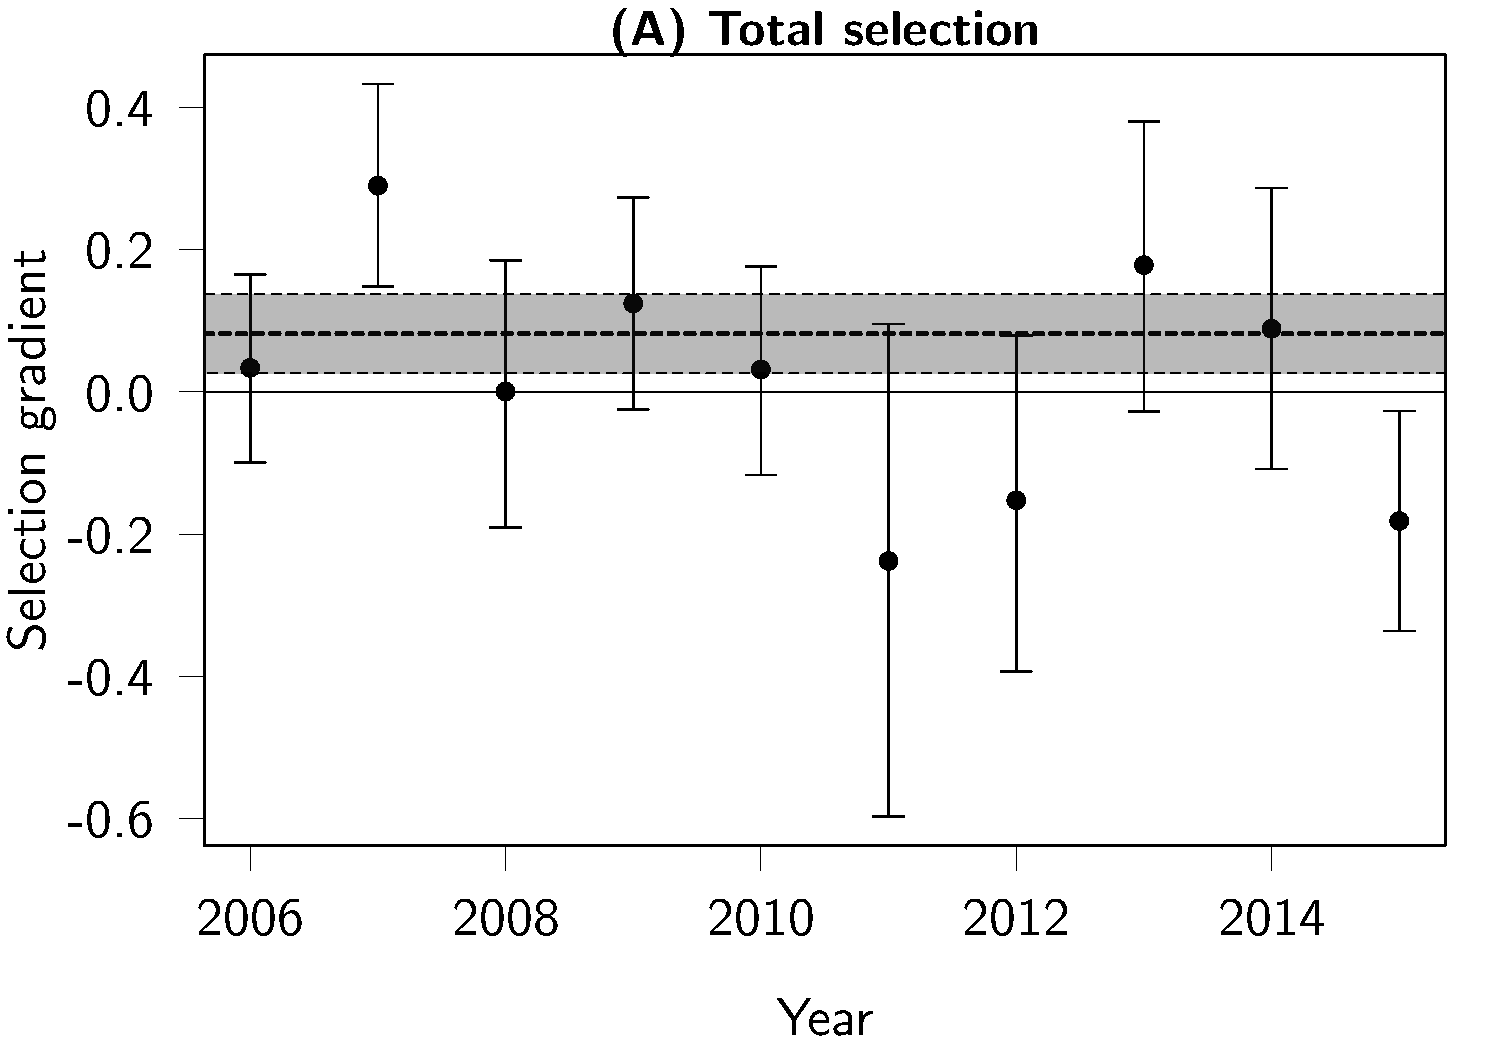
\includegraphics[width=0.5\textwidth]{FiguresFluSel/SelByYear-1}
	
	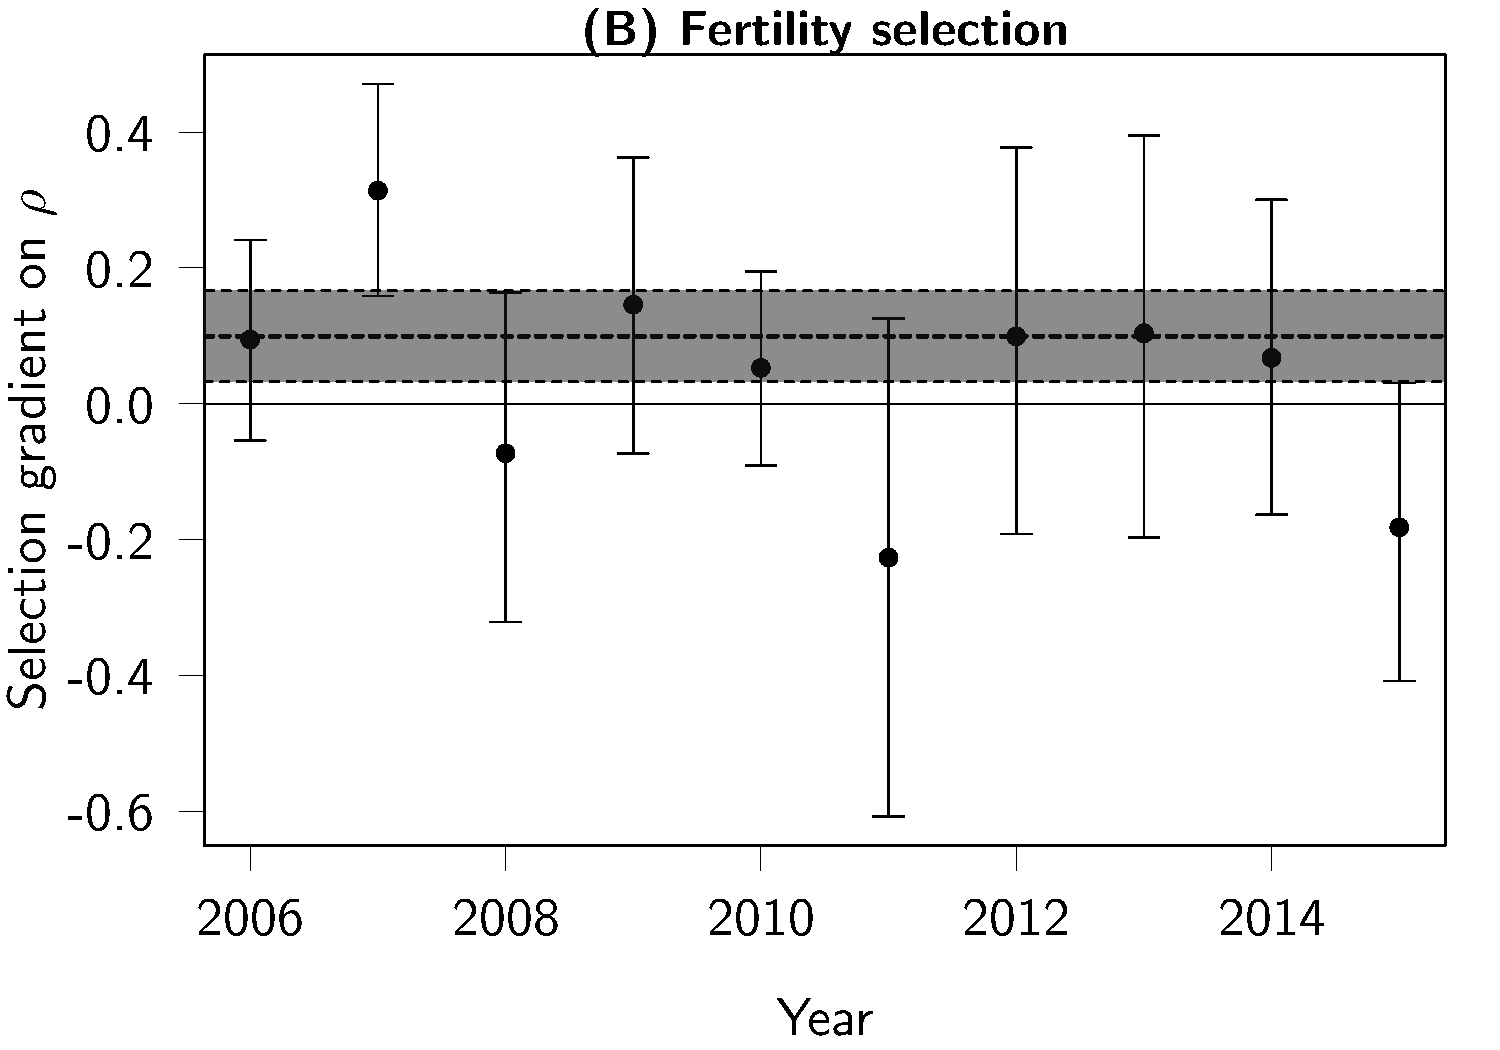
\includegraphics[width=0.5\textwidth]{FiguresFluSel/SelByYearRho-1}
	
	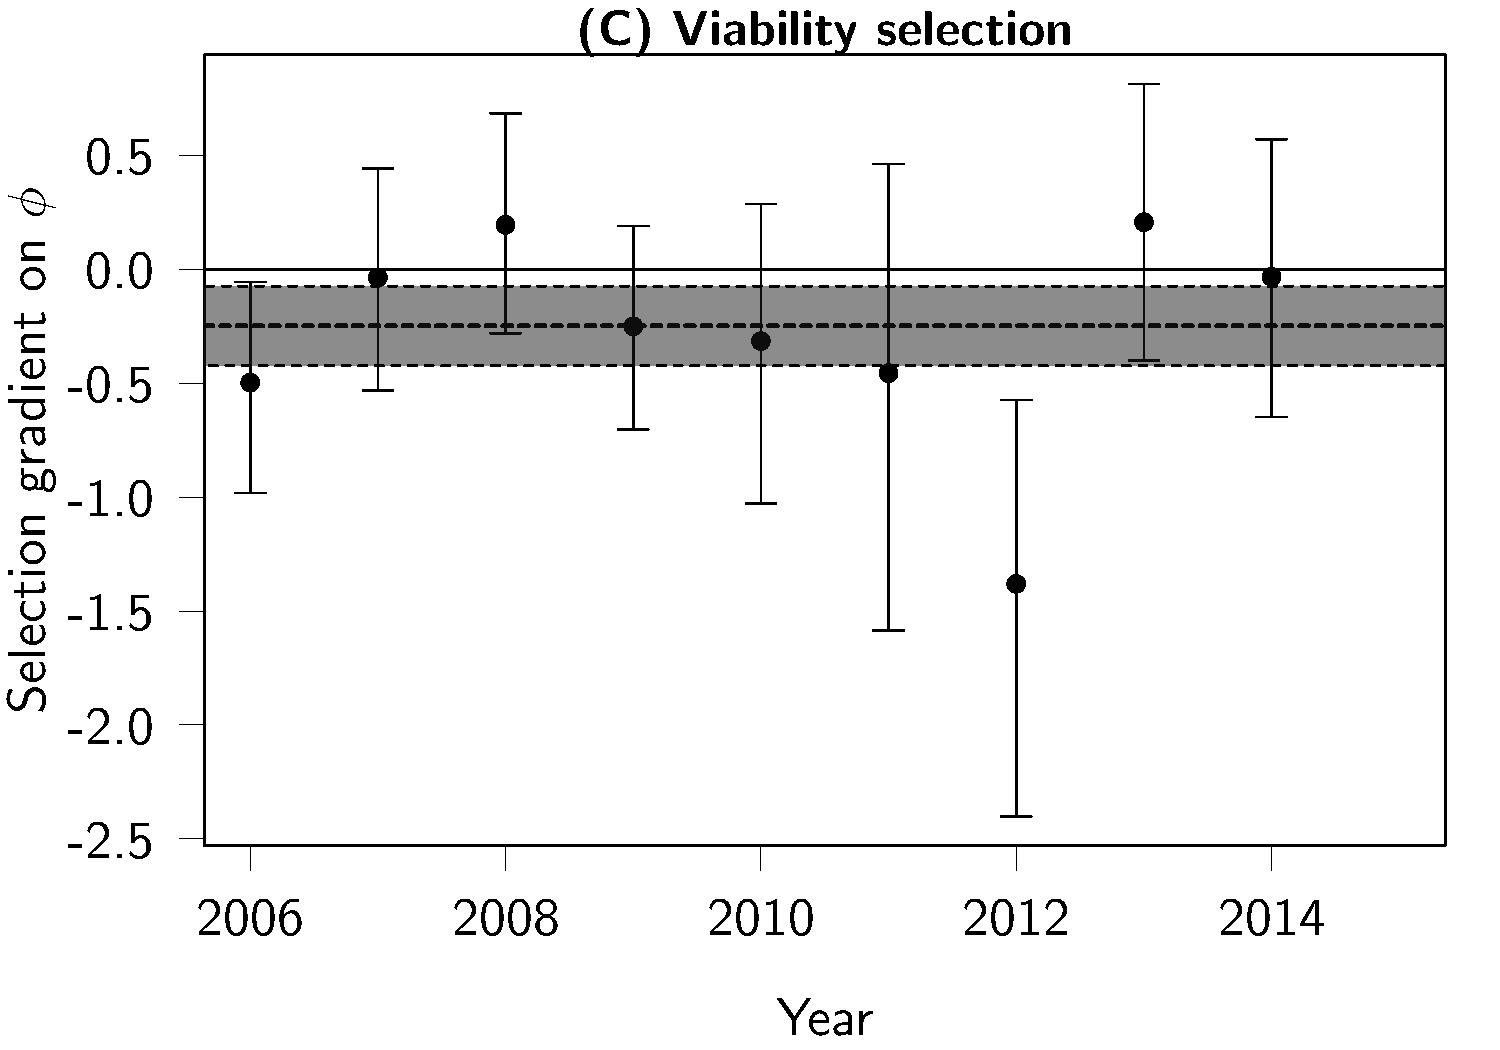
\includegraphics[width=0.5\textwidth]{FiguresFluSel/SelByYearPhi-1}
	\caption{Estimates of overall, viability and fertility selection gradients, year-by-year and across all years. (A) Selection was estimated as the slope of absolute annual fitness (ARS + twice survival) on body mass, on the transformed scale of a Poisson GLM. (B) Selection was estimated as the slope of survival on body mass, on the transformed scale of a binomial GLM. (C) Selection was estimated as the slope of annual reproductive success on body mass, on the transformed scale of a Poisson GLM.
	Year-by-year estimates (black dots with 95\%CI error bars) were obtained by fitting separate GLMs for each year. The overall estimate (dashed line with 95\%CI as a grey polygon) was produced by pooling all years together.}
	\label{fig:yearSel}
\end{figure}

% latex table generated in R 3.2.4 by xtable 1.8-2 package
% Wed May 04 15:30:00 2016
\begin{table}[ht]
{\centering
\caption{\textbf{Selection and temporal variation in selection for total selection ($F$), fertility selection ($\rho$) and viability selection ($\phi$).}}
\label{Test_table}
\begingroup\footnotesize
\begin{tabular}{cccccccc}
\toprule
	Selection & $\beta_z$ (SE)	&	SD$_\text{year}$&	$\overline{\text{SE}_\text{year}}$ & $\beta_{z}^{\prime}$ (SE) & $\sigma_{\zeta}$ 95\%CI & p($\sigma_{\zeta}>0$) & $\abs{\beta_{z}^\prime}/\sigma_{\zeta}$\\
	\midrule  
Total &	0.082 (0.028) & 0.167 & 0.097 & 0.036 (0.044) & 0.117 [0.063;0.218]			& $8\cdot10^{-6}$ 			& 0.309\\ 
Fertility &	0.1 (0.034) & 0.160 & 0.117 & 0.052 (0.044) & 0.111 [0.053;0.212]		& $3\cdot10^{-4}$		& 0.466 \\ 
Viability &	-0.248 (0.089) & 0.484 & 0.319 & -0.217 (0.098) & 0.109 [0;0.425] & $0.36$ & 1.998 \\ 
\bottomrule  
  \end{tabular}
	\label{tab:varsel}
\endgroup}
\footnotesize

Notes: $\beta_z$ is the selection gradient across all years, as estimated from a Generalized Linear Model (GLM),  given with its standard error (SE) ; SD$_\text{year}$ is the standard deviation of selection gradients estimated from year-specific GLMs; $\overline{\text{SE}_\text{year}}$ is the mean standard error on those year-by-year estimates; $\beta_{z}^{\prime}$ is the selection gradient on an average year, estimated from a random regression Generalized Linear Mixed Model (GLMM), given with its standard error; $\sigma_{\zeta}$ is the standard deviation in selection, estimated from this random regression GLMM, given with 95\% confidence interval computed by likelihood profiling; p($\sigma_{\zeta}>0$) is the $p$-value from a likelihood ratio test for the significance of $\sigma_{\zeta}$; $\abs{\beta_{z}^\prime}/\sigma_{\zeta}$ is the ratio of the absolute median year selection over the standard deviation in selection, and indicates the likelihood of absence of reversal in the direction of selection.
\end{table}
%%%%%%%%%%%%%%%%%%%

\subsection*{Statistical significance of variation in selection}
Fitting equation \ref{eq:modRR}, we estimated $\sigma_{F,\zeta} = 0.117$ (95\%CI [0.063;0.218]).
Allowing for annual variation in the selection gradient significantly improved the fit of the model 
($\Delta$log-likelihood = 9.3, one-sided $\chi^2=18.59$, df=1, $p$=$8\cdot10^{-6}$). Fitting a non-zero covariation between the random intercept and the random slope did not change the likelihood of the model ($\Delta$log-likelihood = 1.3, two-sided $\chi^2=2.69$, df=1, $p$=0.10). Given $\abs{\beta_{z}^\prime}/\sigma_{\zeta}=0.309$, the reversal of selection is very likely (table \ref{tab:varsel}).

Variation in fertility selection was estimated as $\sigma_{\rho,\zeta}=0.111$ (95\%CI [0.053;0.212]), which is larger than the median selection gradient ($\beta_{\rho,z}=0.052$ SE$=0.044$). Allowing for fluctuating fertility selection improved significantly the fit of the model to the data ($\Delta$log-likelihood = 6.1, one-sided $\chi^2=12.13$, df=1, $p$=$3\cdot10^{-4}$). There however was little support for fluctuation in viability selection (table \ref{tab:varsel}): Variance in viability selection was not significantly different from zero ($\sigma_{\phi,\zeta}=0.109$; 95\%CI [0;0.425]), accounting for variation in viability selection did not significantly improve the fit of the model ($\Delta$log-likelihood = 0.07, one-sided $\chi^2=0.13$, df=1, $p$=0.36), and the reversal of viability selection was unlikely.

\subsection*{Fluctuation of evolution}
There was a small but significant amount of additive genetic variation in our proxy of annual fitness: On the latent scale of the Poisson model, the additive genetic variation was estimated to be $0.028$ $[0.001;0.082]$. On the scale of the data, this translates into an additive genetic variation of $0.052$ $[0.001;0.105]$ and a heritability of fitness of $1.18\%$ $[0.03\%; 3.17\%]$. This is comparable to the heritability of life-time fitness in \cite{Bonnet2016}, which used a lifetime rather than annual measure of fitness. 

We found significant additive genetic variation in age-corrected mass ($1.99$ g$^2$ [0.91;2.68]; heritability = 17\% [10\%;25\%]). As already shown in \cite{Bonnet2016}, the evolutionary trend from 2006 to 2014 was toward smaller breeding values for mass (Fig. \ref{fig:evolsmooth}). There is however some visual indication of a stabilization and possibly a reversal of evolution in the last two years. 


\begin{figure}[ht]
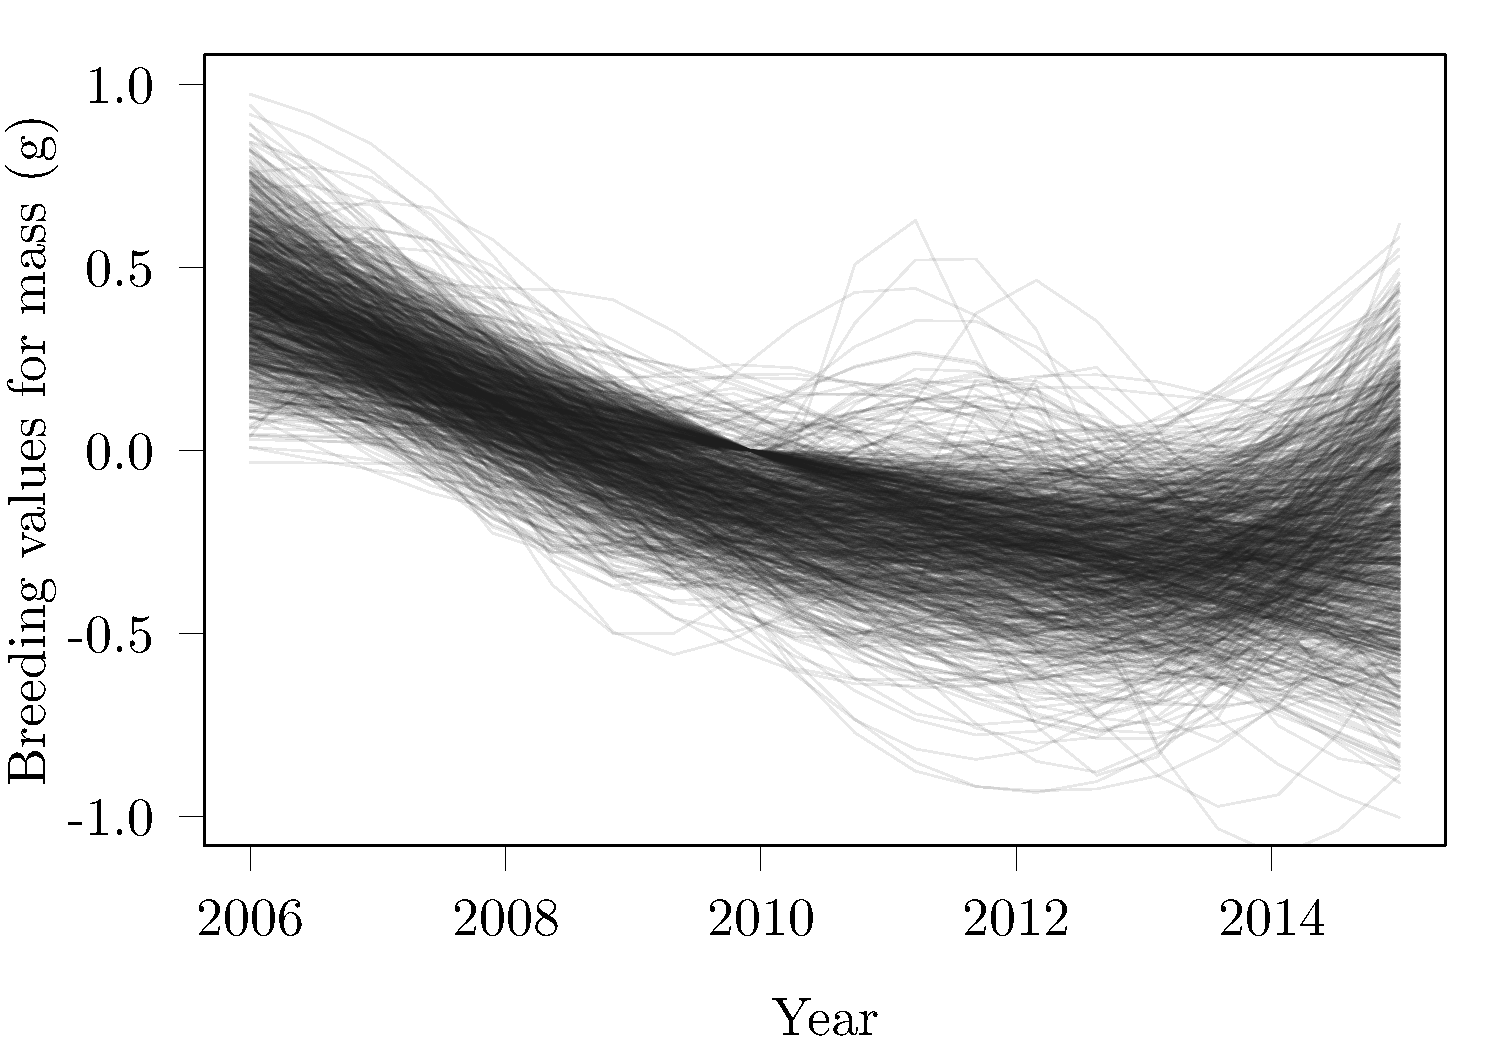
\includegraphics[width=\textwidth]{FiguresFluSel/EvolSmooth-1}
\caption{Temporal dynamics of mean breeding value for mass. Each line was obtained from a different MCMC posterior sample, by fitting a time-spline to the mean of estimated breeding values among individuals alive in any given year.}
\label{fig:evolsmooth}
\end{figure}

The same pattern emerges when looking at the posterior distribution of change in breeding values between any two successive years (Fig. \ref{fig:evoldiff}). None of the year-to-year changes are statistically different from zero (Fig. \ref{fig:evoldiff}), but because they are largely negative or null, they sum up to a strongly negative and statistically significant trend from 2006 to 2014 \parencite{Bonnet2016}. Similarly, although none of the observed changes are stronger than what could be expected due to drift alone (Fig. \ref{fig:evoldiff}), drift cannot explain the cumulative change \parencite{Bonnet2016}.
 
\begin{figure}[ht]
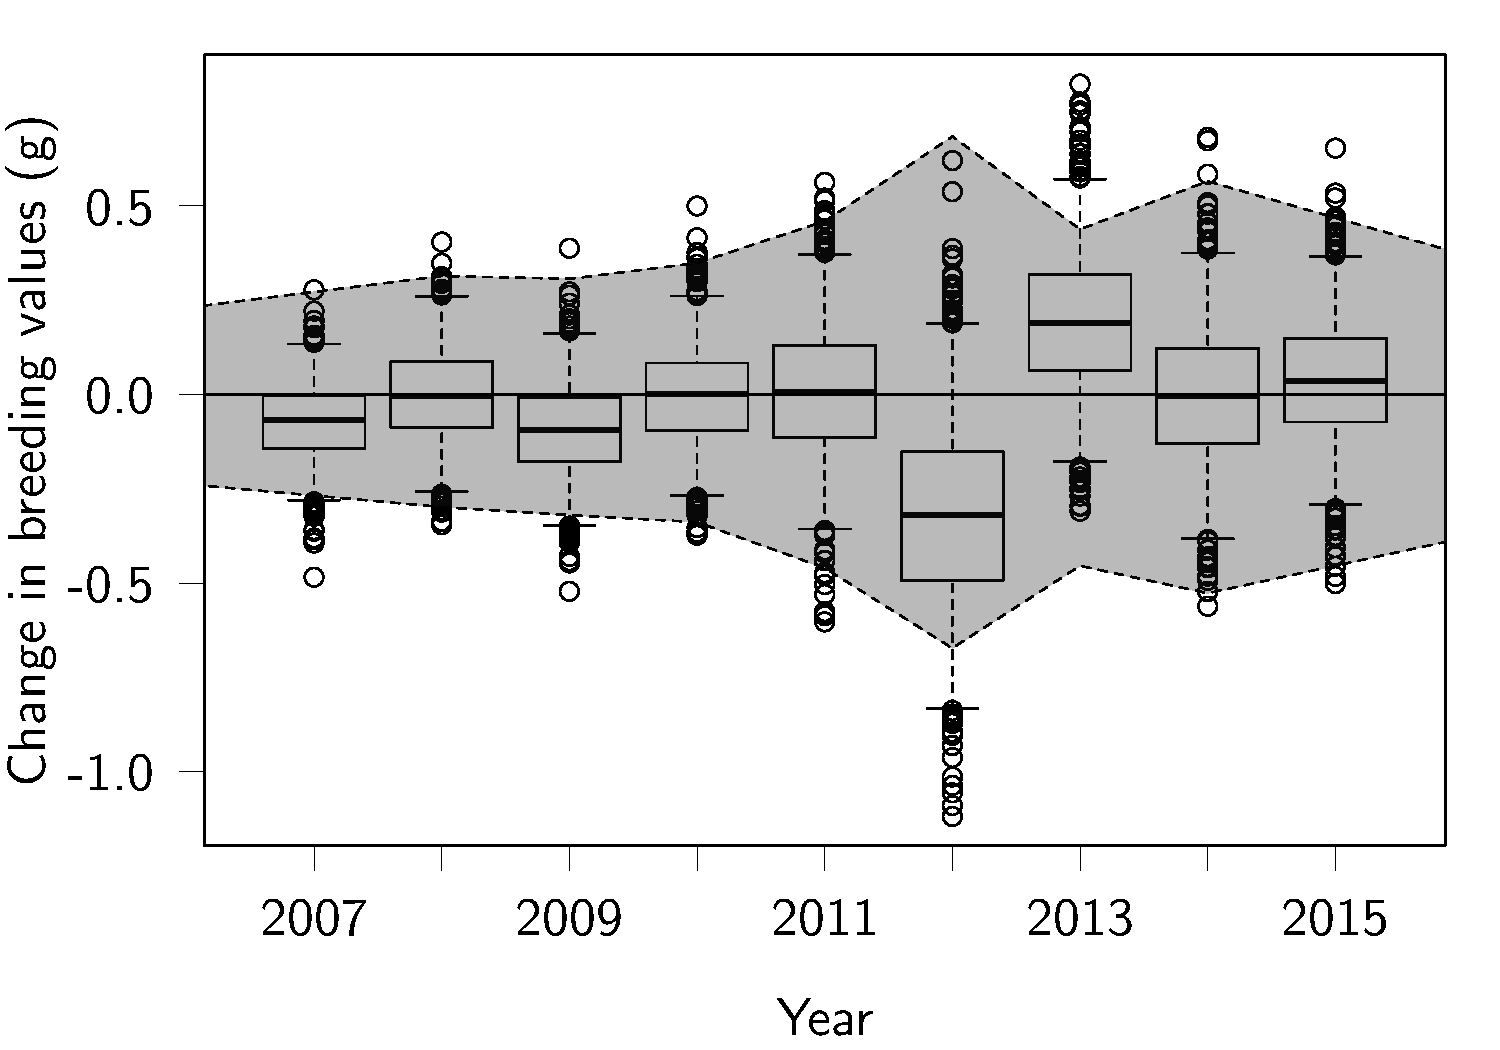
\includegraphics[width=\textwidth]{FiguresFluSel/EvolDiff-1}
\caption{Posterior distribution of the change in breeding values for mass relative to the mean in the previous year, and the range of change possible due to genetic drift. For each posterior sample of the estimated breeding values, we computed the difference between the mean breeding value of individuals alive in year $t$ and individuals alive in year $t-1$. Box plots show the median, the first and third quartiles, quantiles 2.5\% and 97.5\% and outliers. The grey envelope shows the 95\% interval of year-to-year evolution simulated with drift only.}
\label{fig:evoldiff}
\end{figure}

\subsection*{From selection to evolution}

As discusses above, the correlation between selection gradients and change in breeding values from one year to the next is estimated with a lot of uncertainty and is not statistically significantly different from zero. Nevertheless, the most likely value was positive (mode 0.36, 95\%CI $[-0.39; 0.64]$).

As expected, in years with positive selection (based on selection gradients from year-by-year GLMs, see above), the selection gradient reconstructed from our trivariate animal model was positive, while it was negative for years with negative selection gradients (fig. \ref{fig:betas}). Importantly however, the genetic gradients were negative in both groups of years (fig. \ref{fig:betas}) and did not differ from each other ($\beta_{A+}-\beta_{A-} = -0.004$, 95\%CI$ [-0.080;0.076]$, $p_{MCMC}=0.91$). On the other hand, the environmental gradients differed from each other ($\beta_{E+}-\beta_{E-} = 0.075$, 95\%CI$ [0.038;0.137]$, $p_{MCMC}<0.001$), with $\beta_{E+}$ being significantly positive, and $\beta_{E-}$ slightly negative.
Moreover, during years of positive selection, the genetic and environmental gradients were of opposite sign (fig. \ref{fig:betas}), and significantly different ($\beta_{A+}-\beta_{E+} = -0.123$, 95\%CI[-0.218;-0.028], $p_{MCMC}=0.006$).
On the other hand, during years of negative selection, the genetic and environmental gradients were both negative (fig. \ref{fig:betas}), and not significantly different ($\beta_{A-}-\beta_{E-} = -0.010$, 95\%CI[-0.138;-0.058], $p_{MCMC}=0.424$). Finally, the genetic correlation between mass in positive selection years and mass in negative selection years was strong and positive (0.82, 95\%CI $[0.46; 0.93]$).

\begin{figure}[ht]
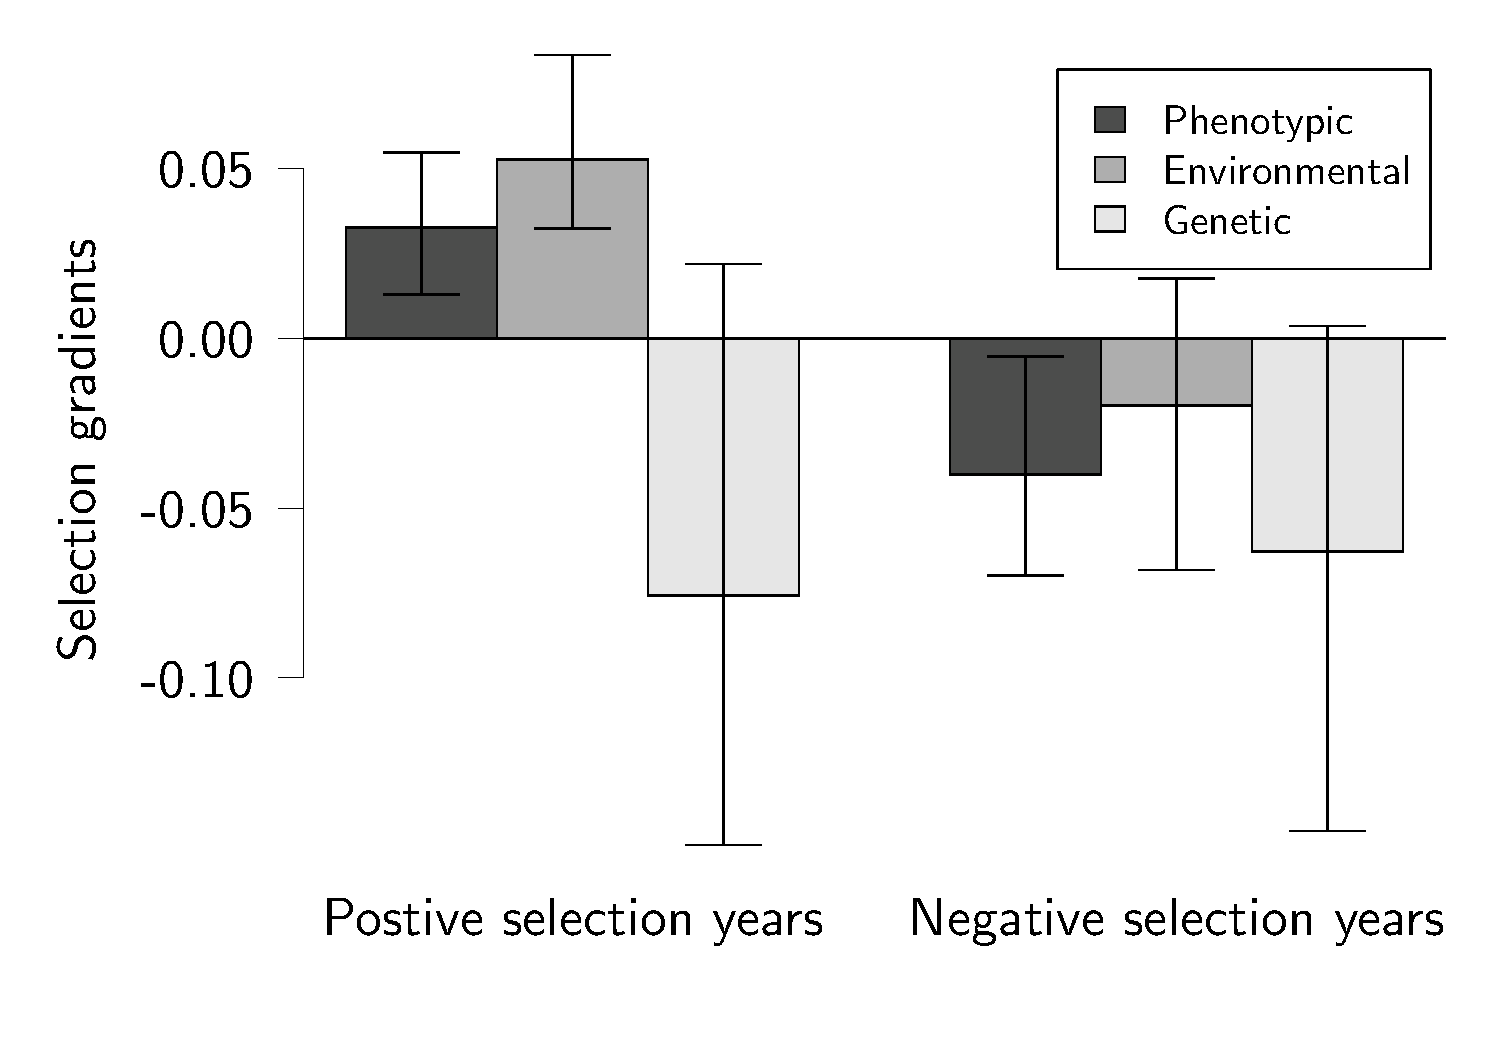
\includegraphics[width=\textwidth]{FiguresFluSel/Betas-1}
\caption{Phenotypic selection gradients and their decomposition into environmental and genetic gradients for years with positive selection on mass and for years with negative selection on mass. Error bars show 95\% confidence intervals.}
\label{fig:betas}
\end{figure}

\section*{Discussion}
Here we have shown that selection on body mass fluctuates in a natural population of snow voles. Fluctuations in total selection originate from changes in fertility rather than viability selection. 
In addition, we have shown that body mass was genetically evolving in this population, and that the rate and direction of evolution were relatively steady. As a consequence, changes in the direction of phenotypic selection did not result in concordant changes in the direction of evolution.

Below, we discuss the methodological challenges to studying the variation in selection and evolution, and highlight our contributions to their resolution. We then clarify why the signs of selection and evolution can be different even though the temporal variations in selection and in evolution are likely to be correlated. We discuss what our analyses can, and cannot, tell about the mechanisms of fluctuating selection, and what is needed to go beyond. 
Finally, we discuss the importance of the time-scale when studying variation in selection and evolution.

\subsection*{The modelling of evolution and selection}
The random regression method, proposed by \cite{Morrissey2012flusel} and developed further by \cite{Chevin2015b} provides a statistically rigorous way to quantify and test for the significance of variation in selection \parencite{Chevin2015b}. On its own, however, a random regression does not address the evolutionary relevance of fluctuating selection. To establish its evolutionary relevance, two additional issues need to be investigated: (i) Variation in the strength of selection will reverse the direction of evolution only if it fluctuates not only in strength, but also in direction (see Figure \ref{fig:concept}B and C); (ii) Furthermore, selection does not always lead to a genetic response to selection \parencite{Rausher1992, Morrissey2010, Merila2001}, and fluctuating selection might have no influence on evolutionary dynamics (see Figure \ref{fig:concept}D).

To address the first issue, we considered how the distribution of selection, estimated by a random regression, is located relative to zero. If this distribution is centred around zero, selection reversal must be frequent, while if the distribution does not overlap much with zero, selection reversal must be rare.
We evaluated the likelihood of selection reversal by calculating the ratio of the absolute median selection gradient over the standard deviation of selection gradients ($\abs{\beta_{z}^\prime}/\sigma_\zeta$). Reversal becomes less likely as this ratio increases.
As only 10 years are included in our analysis, this ratio will not exactly comply with a $Z$-distribution and hence cannot be directly translated into a probability. Nevertheless, it gives a qualitative assessments of the likelihood of reversal and it could be developed further into a more quantitatively rigorous measure.

To address the second issue, we estimated the coupling between variation in selection and variation in  genetic change. While we were able to satisfactorily show that selection and evolution are uncoupled, the exercise proved to be challenging. In a first approach, we computed the correlation between selection and year-to-year changes in breeding values by relating the full distribution of the change in BLUPs for breeding values to point estimates of selection gradients. Therefore, the uncertainty accompanying the selection estimates was not propagated to this correlation. This in contrast to the trivariate animal model, which estimates selection and evolution within the same model. Consequently, this approach allows  to integrate the uncertainty in both selection and evolution when comparing genetic and environmental gradients, and to take into account the non-independence of their posterior distributions. Unfortunately however, this multivariate approach is particularly data-hungry. Because the snow vole population is too small to estimate year-specific genetic parameters, we were forced to group years with negative and positive selection. Nevertheless, whenever the population size allows for it, we advocate the use of year-specific multivariate animal models for the investigation of the question at hand.

\subsection*{Uncoupling of selection and evolution}
We found that both evolution and viability selection did not fluctuate and were always negative, whereas 
fertility selection fluctuated significantly between positive and negative values (table \ref{tab:varsel}, figure \ref{fig:evolsmooth}). 
This is inline with our previous finding that in this population, directional evolution towards lower body mass is driven by viability rather than fertility selection \parencite{Bonnet2016}. Together, this implies that evolution and total selection are partly uncoupled in this system, and in particular that their signs do not match. 

Nevertheless, evolution is not completely independent of selection. While we do not observe a significant correlation between selection and evolution among years\textemdash probably because of strong genetic drift\textemdash the most likely value is positive (see Results). 
Simple algebra shows that a positive correlation is indeed expected. For a trait $z$, a selection gradient is the ratio of the phenotypic covariance between trait and relative fitness, over the phenotypic variance in the trait:
\begin{equation*}
\beta_P = \frac{\sigma_P(z, F)}{\sigma^2_P(z)} \text{.}
\end{equation*}
Assuming a simple quantitative genetic model, $z$ can be additively decomposed into additive genetic effects and environmental effects $z = a + e$, so that there is no correlation or interaction between the genetic effects and the environmental effects. The phenotypic covariance ($\sigma_P(z, F)$, i.e. the selection differential) can be decomposed into an additive genetic ($\sigma_A(z,F)$) and an environmental covariance ($\sigma_E(z,F)$), because all covariances between additive genetic effects and environmental effects are null. Therefore, the phenotypic selection gradient ($\beta_P$) can be written as:
\begin{equation*}
\beta_P = \frac{\sigma_A(z,F)+\sigma_E(z,F)}{\sigma^2_P(z)} \text{.}
\end{equation*}
According to the Robertson-Price identity \parencite{Robertson1966, Price1970}, $\sigma_A(z,F)$ is the expected rate of genetic change. From this it follows that the phenotypic selection gradient is likely to be positively correlated with evolution (provided the latter is non-zero). Therefore, although their signs are opposite, years with more positive selection gradients go with less negative genetic change, and vice versa. 

\subsection*{The mechanisms of fluctuation}
Although our random regression and quantitative genetic models give a thorough description of the dynamics of selection and evolution in this population, they do not provide direct insight into the mechanisms underlying these dynamics. We have shown that selection fluctuates, and thus that the relationship between mass and fitness changes at the population level, but what does this tell us about the dynamics of the fitness landscape? Different processes may lead to the same distribution of directional selection gradients, and based on the analysis of selection gradients alone it is difficult to distinguish fluctuations due to a moving fitness optimum from those due to a change in the distribution of phenotypes among years \parencite{Chevin2014}. The latter may play a role as we find substantial variation between years in both the mean phenotype (ranging between 38.6 g and 40.6 g) and its standard deviation (ranging between 3.1 g and 4.4 g).

Indirectly we can nevertheless gain some insights into the ecological drivers of variation in selection. If the environmental variance in fitness can be interpreted as the environmental variance in individual quality \parencite[see][for a discussion of individual quality in an evolutionary context]{Wilson2010a}, when applied to body mass we could consider this environmental covariation to capture variation in body condition. Although this is nothing more than a reformulation, it can promote a better understanding of the nature and the dynamics of the environmental covariation between body mass and fitness. In the snow voles, in agreement with the interpretation of environmental covariation as body condition, the environmental covariation is either positive or null (depending on years, see Fig. \ref{fig:betas}) but never significantly negative.
Changes in the environmental covariation seems to be primarily related to the fluctuation of fertility selection. Indeed, fertility selection fluctuates, whereas viability selection does not (table \ref{tab:varsel}), and fertility selection is independent of genetic variation for mass \parencite{Bonnet2016}.
It is therefore likely that a favourable territory\textemdash for instance with high food availability and low parasitic prevalence\textemdash increase voles mass and reproductive success simultaneously, that is, increases voles body condition. The amplitude of variation in body condition could depend on the prevalence of parasites or on the availability of good territories, mediated by vole density. More research is needed to test these ideas.

If we are to gain a deeper understanding of the dynamics of the fitness landscape and the ecological drivers of selection, we ultimately need to move beyond the estimation of variance parameters, toward a more mechanistic understanding of the genetic and ecological sources of phenotypic variation and their covariance with fitness \parencite{Morrissey2012flusel}. However, good examples of where we know the ecological driver of variation in selection are scarce. Some notable exceptions are beak size in Darwin finches \parencite{Grant2002} and reproductive timing in great tits \parencite{Husby2011}. Both of these, as well as the present study, rely on individual-based long-term monitoring, difficult and costly to upkeep, but necessary to disentangle the causes and consequences of selection in natural populations \parencite{Clutton-brock2010}. 
%An alternative could consist in identifying 
 %Furthermore, some insight into the causes of fluctuating selection and its evolutionary consequences could be gained from time-series of Mendelian morphs \parencite{Fisher1947} or allele frequencies across the genome \parencite{LeRouzic2015}, which might help to identify the pathways and traits related to fluctuating selection, and from there infer the ecological drivers. In practice, however, inferring fluctuating selection and evolution from molecular data is still a statistical challenge, as it requires an exceptional quantity and quality of data even for traits with a simple genetic architecture \parencite{LeRouzic2015}.

\subsection*{Time-scale} 
Despite fluctuations in the strength and direction of phenotypic selection, the rate and direction of evolution was constant over the course of the study period. Thereby our findings are at odds with the idea that fluctuating selection causes short-term evolutionary stasis. Nevertheless, fluctuating selection may be a driver of short-term evolutionary dynamics in other natural populations, where the selection measured by regression-based methods is causal and not dominated by an environmental covariation between traits and fitness. Moreover, it is unlikely that fluctuating selection will not be evolutionary relevant on some longer time scales, in the snow vole population and in other populations.  Over geological time scales, bounded fluctuations of phenotypic evolution are increasingly recognized as the signature of fluctuating selection, rather than sampling variation around a real evolutionary stasis \parencite{Uyeda2011, Voje2015}. Unless the environment is perfectly constant, causal selective pressures are likely to change over longer time periods, whether the fitness landscape changes, or whether the phenotypic distribution changes through response to selection or phenotypic plasticity. 

Any study might not detect fluctuating selection, or might not find an evolutionary role for fluctuating selection, because the time frame is too short to observe significant changes in the environment, but also because the time unit at which selection is estimated is too long, smoothing out very short changes in selection and the rate of genetic change. Thus, in the snow vole population, adaptive evolution and the causal selective pressure causing it are probably related to a short-term climatic anomaly over a decade and likely to be reversed by global climate change \parencite{Bonnet2016}. Moreover, the causal selective pressure varies within a year: selection is null early in the reproductive season and increases throughout summer \parencite{Bonnet2016}.
Therefore, our point is not to say that fluctuating selection has no evolutionary relevance in general. Instead, we warn against interpreting any phenotypic fluctuating selection in term of fluctuating evolution. 

\subsection*{Conclusion} 

Our results highlight the danger of relying on temporally replicated phenotypic estimates of selection to understand and predict the evolutionary dynamics of natural populations. As the dynamics of selection and evolution can be uncoupled on certain time scales, fluctuating selection does not necessarily provide a reasonable explanation for evolutionary stasis. Instead, quantifying the evolutionary relevance of fluctuating selection requires a joined analysis of selection and evolution.  

%%%%%%%%%%%%%%%%%%%%%%%%%%%%%%%%%%%%%%%%%
\section*{Acknowledgments}
Thanks to Jarrod D. Hadfield, Lukas F. Keller, Marc K\'{e}ry and Pirmin Nietlisbach for comments on earlier versions of this work. Thanks to the many field helpers over 10 years. Weather data were provided by MeteoSwiss. The snow vole monitoring was authorised by the \textit{Amt f\"{u}r Lebensmittelsicherheit und Tiergesundheit}, Chur, Switzerland. T.B. is funded by a Swiss National Science Foundation project grant (\verb|31003A_141110|) awarded to EP. 

\printbibliography[heading=subbibliography]